%%This is a very basic article template.
%%There is just one section and two subsections.
\documentclass{llncs}

\usepackage{tikz}
\usetikzlibrary{intersections,decorations.pathreplacing,fit,calc,3d,positioning,shapes.geometric,matrix}
\pgfdeclarelayer{background}
\pgfsetlayers{background,main}

\usepackage[range-phrase = --]{siunitx}
\usepackage{booktabs,amsmath,amssymb,dsfont,etoolbox,multirow,calc,printlen}
\usepackage{hyperref}
\usepackage{subfigure}
\usepackage{todonotes,comment}

\robustify\bfseries % requires etoolbox
\newcommand{\minitab}[2][l]{\begin{tabular}{#1}#2\end{tabular}}

\usepackage{array}
\newcolumntype{C}[1]{>{\centering\let\newline\\\arraybackslash\hspace{0pt}}m{#1}}

\title{Deep Convolutional Encoder Networks for Multiple Sclerosis Lesion
Segmentation}

\author{%
***
% Tom Brosch\inst{1,3} \and
% Youngjin Yoo\inst{1,3} \and
%David K.B. Li\inst{2,4} \and
%Anthony Traboulsee\inst{3,4} \and
% Roger Tam\inst{2,3}
}
% \index{Brosch, Tom}
% \index{Yoo, Youngjin}
% \index{Li, David K.B.}
% \index{Traboulsee, Anthony}
% \index{Tam, Roger}

\institute{%
% Department of Electrical and Computer Engineering, UBC
***
\and
% Department of Radiology, UBC
***
% % Division of Neurology, UBC
\and
% MS/MRI Research Group, University of British Columbia, Vancouver, Canada
***
}

\newcommand{\vect}[1]{\vec{#1}}
\newcommand{\thetas}{\vec{\theta}}
\newcommand{\mus}{\vec{\mu}}
\newcommand{\data}{\mathcal{D}}
\newcommand{\given}{\mid}
\DeclareMathOperator{\sigm}{sigm}
\DeclareMathOperator{\conj}{conj}
\DeclareMathOperator{\fft}{fft}
\DeclareMathOperator{\ifft}{ifft}
\newcommand{\R}{\ensuremath{\mathds{R}}}
\newcommand{\Q}{\ensuremath{\mathds{Q}}}
\newcommand{\N}{\ensuremath{\mathds{N}}}
\newcommand{\E}{\ensuremath{\mathds{E}}}
\newcommand{\I}{\ensuremath{\mathds{I}}}
\newcommand{\F}{\ensuremath{\mathcal{F}}}
\newcommand{\Norm}{\ensuremath{\mathcal{N}}}

\hyphenation{conv-RBM}
\hyphenation{conv-RBMs}
\hyphenation{sconv-RBM}
\hyphenation{sconv-RBMs}

\begin{document}

\maketitle
\setcounter{footnote}{0}
\begin{abstract}

% TODO: mention that we compared different architectures
% TODO: Distinguish from the work of other's more

We propose a novel segmentation approach based on deep multi-layer convolutional
encoder networks with shortcut connections and apply it to the segmentation of
multiple sclerosis (MS) lesions in magnetic resonance images. Our model is a
neural network that consists of two interconnected pathways, a convolutional
pathway, which consists of alternating convolutional and pooling layers and
learns increasingly more abstract and robust image features, and a
deconvolutional pathway, which consists of alternating deconvolutional and
unpooling layers and predicts the final segmentation. The joint training of the
feature extraction and prediction pathways allows for the automatic learning of
features at different scales that are optimized for accuracy for any given
combination of image types and segmentation task. In contrast to previously used
patch-based feature learning approaches and similar to recently proposed neural
network architectures, our model learns features from entire images instead of
from patches, which eliminates patch selection and redundant calculations at the
overlap of neighboring patches and thereby speeds up the training. However,
unlike previous such approaches, our method predicts segmentations of the same
resolution and size as the input images, which makes it more accurate and
eliminates the need for special border handling. We have evaluated our method on
a large data set from an MS clinical trial showing that our method is able to
segment MS lesions more accurately than our previously proposed 3-layer network
and Lesion-TOADS, a widely used and freely available method for the automatic
segmentation of MS lesions.

%In addition, our network also uses a new objective function
%that works well for segmenting underrepresented classes, such as MS lesions.

% We have evaluated our method on the publicly
% available labeled cases from the MS lesion segmentation challenge 2008 data set,
% showing that our method performs comparably to the state-of-the-art. In
% addition, we have evaluated our method on the images of 500 subjects from an MS
% clinical trial and varied the number of training samples from 5 to 250 to show
% that the segmentation performance can be greatly improved by having a
% representative data set.
\end{abstract}

% Note that keywords are not normally used for peerreview papers.
\begin{IEEEkeywords}
Segmentation, multiple sclerosis lesions, magnetic resonance imaging (MRI), deep
learning, convolutional neural networks, machine learning 
\end{IEEEkeywords}

\section{Introduction}

\IEEEPARstart{M}{ultiple}
sclerosis (MS) is an inflammatory and demyelinating disease of the central
nervous system with pathology that can be observed in vivo by magnetic resonance
imaging (MRI). MS is characterized by the formation of lesions, primarily
visible in the white matter on conventional MRI. Imaging biomarkers based on the
delineation of lesions, such as lesion load and lesion count, have established
their importance for assessing disease progression and treatment effect.
However, lesions vary greatly in size, shape, intensity and location, which
makes their automatic and accurate segmentation challenging.

% Generative model was dictionary learning and sparse coding. Might extend
% clustering a little bit if need be.

Many automatic methods have been proposed for the segmentation of MS
\mbox{lesions} over the last two decades \cite{garcia2013review}, which can be
classified into unsupervised and supervised methods. Unsupervised methods do not
require a labeled data set for training. Instead, lesions are identified as an
outlier of, e.g., a subject specific generative model of tissue intensities
\cite{vanleemput2001,tomas2015,schmidt2012automated,roura2015}, or a generative
model of image patches representing a healthy population \cite{weiss2013}.
Alternatively, clustering methods have been used to segment healthy and lesion
tissue, where lesions are modelled as a separate tissue class
\cite{shiee2010topology,sudre2015}.
In many methods, spatial priors of healthy tissues are used to reduce false
positives. For example, in addition to modelling MS lesions as a separate
intensity cluster, Lesion-TOADS \cite{shiee2010topology} employs topological and
statistical atlases to produce a topology-preserving segmentation of all brain
tissues.
%, while the expectation-maximization segmentation (EMS)
%\cite{vanleemput2001} method uses a Markov random field (MRF) to produce a
%spatially consistent segmentation.
% TODO: maybe remove or reword the EMS MRF.

% To account for the variability of intensity distributions for different
% subjects and scanning sequences, Sudre et al used Bayesian model selection to
% select the most appropriate statistical model for each healty tissue and
% lesion class.
To account for local changes of the tissue intensity distributions,
Tomas-Fernandez et al. \cite{tomas2015} combined the subject-specific model of
the global intensity distributions with a voxel-specific model calculated from a
healthy population, where lesions are detected as outliers of the combined
model. A major challenge of unsupervised methods is that outliers are often not
specific to lesions and can also be caused by intensity inhomogeneities, partial
volume, imaging artifacts, and small anatomical structures such as blood
vessels, which leads to the generation of false positives. To overcome these
limitations, Roura et al. \cite{roura2015} employed an additional set of rules
%TODO: Can we add an adjective or two to make this more specific? (rules)
to remove false positives, while Schmidt et al. \cite{schmidt2012automated} used
a conservative threshold for the initial detection of lesions, which are later
grown in a separate step to yield an accurate delineation.


% Outlier of a subject-specific generative model of healthy tissue intensities
% [ems] or outlier of image patches representing a healthy population [weiss].
% Or modelled as a separate cluster [shiee,sudre].

%Other methods derive a tissue segmentation using clustering methods and model
%lesions as a separate cluster \cite{shiee2010topology,sudre2015}. The
%intensities of healthy and lesion tissue might can not always be modelled by a
%single centroid or multivariate Gaussian. Sudre et al. have used Bayesian
%inference to select the most appropriate statistical model to represent each
%tissue cluster.

% Instead, lesions are identified as an intensity outlier class using, e.g.,
% clustering methods \cite{shiee2010topology} or generative models
% \cite{weiss2013}. In many methods, spatial priors of healthy tissues are used to
% reduce false positives. For example, in addition to modelling MS lesions as a
% separate cluster, Lesion-TOADS \cite{shiee2010topology} employs a topological
% and a statistical atlas to produce a topology-preserving segmentation of all
% brain tissues.

Current supervised approaches typically start with a set of features, which can
range from small and simple to large and highly variable, and either predefined
by the user \cite{geremia2010,guizard2015,subbanna2015} or gathered in a feature
extraction step such as by deep learning \cite{yoo2014}. Voxel-based
segmentation algorithms \cite{geremia2010,yoo2014} feed the features and labels
of each voxel into a general classification algorithm, such as a random forest
\cite{breiman2001}, to classify each voxel and to determine which set of
features are the most important for segmentation in the particular domain.
% TODO: introduce MRF better
Voxel features and the labels of neighboring voxels can be incorporated into
Markov random field-based (MRF-based) approaches
\cite{subbanna2009,subbanna2015} to produce a spatially consistent segmentation.
As a strategy to reduce false positives, Subbanna et al.
\cite{subbanna2015} combined a voxel-level MRF with a regional MRF, which
integrates a large set of intensity and textural features extracted from the
regions produced by the voxel-level MRF with the labels of neighboring nodes of
the regional MRF.
Library-based approaches leverage a library of pre-segmented images to carry out
the segmentation. For example, Guizard et al.
\cite{guizard2015} proposed a segmentation method based on an extension of the
non-local means algorithms \cite{coupe2011}. The centers of patches at every
voxel location are classified based on matched patches from a library containing
pre-segmented images, where multiple matches are weighted using a similarity
measure based on rotation-invariant features.

% Current supervised approaches typically start with a simple or large set of
% features, either predefined by the user
% \cite{geremia2010,guizard2015,subbanna2015} or gathered in a feature extraction
% step such as by deep learning \cite{yoo2014}, which is followed by a separate
% training step with labeled data to determine which set of features are the most
% important for segmentation in the particular domain. Alternative approaches were
% proposed by Subbanna et al. and Guizard et al.
% 
% Alternative, start with a simple set of features and derives more complex
% features from regions created by an initial segmentation. \cite{subbanna2015}:
% Combines two MRFs. Initial segmentation carried out by the voxel level MRF that
% uses the image intensities and intensity differences as input features.
% Segmentation is iteratively updated using a regional MRF, where each node uses a
% complex set of intensity and textual feature derived from the regions segmented
% by the voxel level MRF. Distributions of features for each tissue type and
% transitions are learned from training data.
% 
% Guizard et al. \cite{guizard2015} proposed a segmentation method based on an
% extension of the non-local means algorithms \cite{coupe2011}. The centers of a
% patch at every voxel location is classified based on matched patches from a
% library containing pre-segmented images, where multiple matches are weighted
% using a similarity measure based on rotation-invariant features extracted from
% the patches.

% For example, Yoo et al. \cite{yoo2014} proposed performing unsupervised
% learning of domain-specific features from image patches from unlabelled data
% using deep learning.
A recent breakthrough for automatic segmentation using deep learning comes from
the domain of cell membrane segmentation, in which Cire\c{s}an et al.
\cite{Ciresan2012} proposed classifying the centers of image patches directly
using a convolutional neural network (CNN) \cite{LeCun1998} without a dedicated
feature extraction step. Instead, features are learned indirectly within the
lower layers of the neural network during training, while the higher layers can
be regarded as performing the classification, which allows the learning of
features that are specifically tuned to the segmentation task. However, the time
required to train patch-based methods can make the approach infeasible when the
size and number of patches are large.

% TODO: can I add numerical values to it? Mostly my personal experience.

% TODO: Where does this approach fit in, what is the contribution?

Recently, different CNN architectures
\cite{long2015,ronneberger2015,brosch2015,kang2014fully} have been proposed that
are able to feed through entire images, which removes the need to select
representative patches, eliminates redundant calculations where patches overlap,
and therefore these models scale up more efficiently with image resolution. Kang
et al. introduced the fully convolutional neural network (fCNN) for the
segmentation of crowds in surveillance videos \cite{kang2014fully}. However, fCNNs produce
segmentations of lower resolution than the input images due to the successive
use of convolutional and pooling layers, both of which reduce the
dimensionality.
To predict segmentations of the same resolution as the input images, we recently
proposed using a 3-layer convolutional encoder network (CEN) \cite{brosch2015}
for MS lesion segmentation. The combination of convolutional \cite{LeCun1998}
and deconvolutional \cite{zeiler2011} layers allows our network to produce
segmentations that are of the same resolution as the input images.

Another limitation of the traditional CNN is the trade-off between localization
accuracy, represented by lower-level features, and contextual information,
provided by higher-level features. To overcome this limitation, Long et al.
\cite{long2015} proposed fusing the segmentations produced by the lower layers of the network
with the upsampled segmentations produced by higher layers. However, using only
low-level features was not sufficient to produce a good segmentation at the
lowest layers, which is why segmentation fusing was only performed for the three
highest layers.
% TODO: This is unclear. What was wrong with the low-level segmentations? I can
% imagine too many false positives?
Instead of combining the segmentations produced at
different layers, Ronneberger et al. \cite{ronneberger2015} proposed combining
the features of different layers to calculate the final segmentation
directly at the lowest layer using an 11-layer u-shaped network architecture
called u-net. Their network is
% which leverages high-level and low-level features in order to predict
% segmentations that are both robust and accurate.
composed of a traditional contracting path (first half of the u), but augmented
with an expanding path (last half of the u), which replaces the pooling layers
of the contracting path with upsampling operations. To leverage both high- and
low-level features, shortcut connections are added between corresponding layers
of the two paths.
However,
% the successive application of convolutional, pooling, and unpooling layers
% reduces the size of the predicted segmentation by the size of the receptive
% field. This requires special handling of the border regions and limits the
% maximum size of the receptive field.
upsampling cannot fully compensate for the loss of resolution, and special
handling of the border regions is still required.

% Easier to apply than u-net because it does not need padding or cropping of the
% segmentation for training.
% 
% In this paper, we extend our previous framework to include more layers. Our
% model consists of two pathways, a convolutional pathway which consists of
% alternating convolutional and pooling layers and learns increasingly more
% abstract and robust features, and a deconvolutional pathway which consists of
% alternating deconvolutional and unpooling layers. In order for the segmentation
% to be driven by both low-level and high-level features, we introduce shortcut
% connections between layers of the two pathways. Similar to the u-net
% architecture, this allows the segmentation to be driven by both low-level and
% high-level features. In addition, the formalization of shortcut connections
% allows errors to be propagated through the shortcut connections, which in tern
% allows the learning of low-level features that are tuned for segmentation.

% Mention that we compared different architectures

% TODO: differences to u-net, contribution to u-net. U-net more for tissues, our
% method for brain, one structure and we are in 3D. What are new challenges in
% 3D? Runtime and memory.

We propose a new convolutional network architecture that combines the advantages
of a CEN \cite{brosch2015} and a u-net \cite{ronneberger2015}. Our
network is divided into two pathways, a traditional convolutional pathway, which
consists of alternating convolutional and pooling layers, and a deconvolutional
pathway, which consists of alternating deconvolutional and unpooling layers and
predicts the final segmentation. Similar to the u-net, we introduce shortcut
connections between layers of the two pathways. In contrast to the u-net, our
network uses deconvolution instead of upsampling in the expanding pathway and
predicts segmentations that have the same resolution as the input images and
therefore does not require special handling of the border regions. We have
evaluated our method on two widely used publicly available data sets for the
evaluation of MS lesion segmentation methods and a large in-house data set
from an MS clinical trial, with a comparison of network architectures of
different depths and with and without shortcuts\footnote{Where the risk of
confusion is minimal, we will refer to the shortcut connections between two
corresponding layers as a single shortcut (see Fig. 1).}. The results will be
presented in detail in Section~III.

% The results show that increasing depth from three to seven layers
% improves performance, and adding shortcut connections further improves accuracy.
% Overall, our method demonstrates consistently strong segmentation performance
% across a wide range of lesion loads, and in a direct comparison outperforms
% Lesion-TOADS \cite{shiee2010topology}, an established, widely used and freely
% available automatic MS lesion segmentation method.

% There has been a lot of interest in recent years in the machine learning
% community to develop better training methods for CNNs. However, training CNNs
% for medical image segmentation is particularly challenging due to the relatively
% small size of available training sets and the large size of 3D medical images,
% which only allows a few iterations to be used for training and hyperparameter
% tuning. Our second contribution is a comprehensive comparison of different first
% order and second order training method and parameter initialization strategies
% that can serve as a guideline for other researchers for training convolutional
% models for medical image segmentation.

% \item (Analysis of the relationship between regularization and training set
% size to avoid over- and underfitting)

% In this paper, we
% investigate the relationship between training set size and depth of the model on
% the segmentation performance and overfitting and compared the results to a the
% state-of-the-art lesion segmentation method lesion-TOADS, showing that network
% depth can improve segmentation performance for large data sets, but can also
% decrease the performance due to overfitting for smaller training sets, which
% makes network depth a tunable hyperparameter of the model. We've also
% investigated the influence of pre-training on the resulting model, showing that
% although the impact on the performance is minor, it has a big impact on the
% learned features.

% In this paper, we will build on our previous work. Although these networks have
% shown great potential, training of these networks can be difficult. The main
% contribution of this paper is a comprehensive comparison of different training
% strategies and algorithms that can serve as a guideline of how to design and
% train convolutional encoder networks. We have compared different first order and
% second order training methods and found the the right algorithm can have a major
% impact on the performance of the trained network. In addition, we evaluated the
% impact of pre-training and found that pre-training can significantly increase
% classification accuracy by preventing overfitting, if only small data sets are
% available. In addition, we evaluated the impact of the used objective function,
% comparing popular choices with our own objective function.

% We propose a new method for segmenting MS lesions that processes entire MRI
% volumes through a neural network with a novel objective function to
% automatically learn features tuned for lesion segmentation.
% Similar to fully convolutional networks \cite{kang2014fully}, our network
% processes entire volumes instead of patches, which removes the need to select
% representative patches, eliminates redundant calculations where patches overlap,
% and therefore scales up more efficiently with image resolution. This speeds up
% training and allows our model to take advantage of large data sets.
% Our neural network is 

% composed of three layers: an input layer composed of the
% image voxels of different modalities, a convolutional layer \cite{LeCun1998}
% that extracts features from the input layer at each voxel location, and a
% deconvolutional layer \cite{zeiler2011} that uses the extracted features to
% predict a lesion mask and thereby classify each voxel of the image in a single
% operation. The entire network is trained at the same time, which enables feature
% learning to be driven by segmentation performance. The proposed network is
% similar in architecture to a convolutional auto-encoder \cite{masci2011}, which
% produces a lower dimensional encoding of the input images and uses the decoder
% output to measure the reconstruction error needed for training, while our
% network uses the decoder to predict lesion masks of the input images. Due to the
% structural similarity to convolutional auto-encoders, we call our model a
% convolutional encoder network (CEN). Traditionally, neural networks are trained
% by back-propagating the sum of squared differences of the predicted and expected
% outputs. However, if one class is greatly underrepresented, as is the case for
% lesions, which typically comprise less than \SI{1}{\percent} of the image
% voxels, the algorithm would learn to ignore the minority class completely.
% To overcome this problem, we propose a new objective function based on a
% weighted combination of sensitivity and specificity, designed to deal with
% unbalanced classes and formulated to allow stable gradient computations.

\section{Methods}
\label{sec:method}

In this paper, the task of segmenting MS lesions is defined as finding a
function $s$ that maps multi-modal images $I$, e.g., $I = (I_\text{FLAIR},
I_\text{T1}, I_\text{T2})$, to corresponding lesion masks $S$. Given a set of
training images $I_n$, $n \in \N$, and corresponding segmentations $S_n$, we
model finding an appropriate function for segmenting MS lesions as an
optimization problem of the following form
\begin{equation}
\hat{s} = \arg \min_{s \in \mathcal{S}} \sum_n E(S_n, s(I_n)).
\label{eq:segprob}
\end{equation}
where $\mathcal{S}$ is the set of possible segmentation functions, and $E$ is an
error measure that calculates the dissimilarity between ground truth
segmentations and predicted segmentations.

% where $x^{(1)}_1 = I_\text{flair}$, $x^{(1)}_2 = I_\text{t1}$, $x^{(1)}_3 =
%  I_\text{t2}$, and $x^{(1)}_4 = I_\text{prior}$.

% \paragraph{Problem definition}
% \begin{itemize}
% 
% \item Given a set of multi-modal images $I_n = (I_{n, \text{flair}})$ and
% corresponding segmentations $S_n$, we define the task of finding an appropriate
% segmentation algorithm, as the task of finding a function $s$ that maps images
% to their segmentations, i.e. $S_n = s(I_n)$.
% 
% \item Segmentation is a function $s$ that maps an image $I$ to its segmentation
% $S$. That is $S = s(I)$.
% 
% \item Given a set of training images $I_i$ and corresponding segmentations
% $S_i$, we treat finding an appropriate function for segmenting T2 lesions as an
% optimization problem of the following form:
%  \begin{equation} 
% \hat{s} = \arg \max_{s \in \mathcal{S}} \sum_n \text{sim}(S_n, s(I_n)).
% \label{eq:segprob}
% \end{equation}
% where $\text{sim}$ denotes a function that calculates the similarity between
% ground truth segmentations and predicted segmentations, and $\mathcal{S}$ is the
% set of possible functions.
% \end{itemize}

\begin{figure}[tb]
\centering
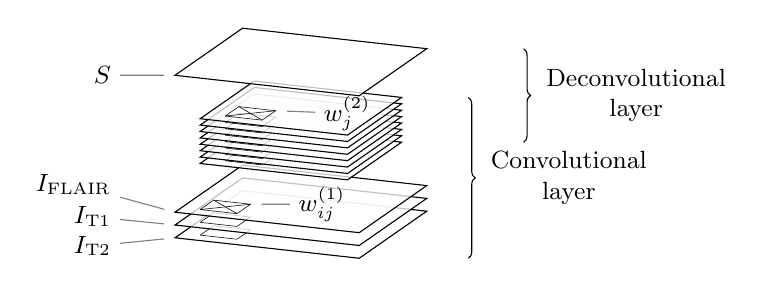
\begin{tikzpicture}[%
scale=0.65,
x  = {(0.9cm,-0.1cm)},
y  = {(0.33cm,0.23cm)},
z  = {(0cm,1cm)}]

\tikzstyle{every node}=[font=\small, inner sep=3pt, align=center]
\tikzstyle{every pin}=[align=center,fill=white]
\tikzstyle{dbnlabel}=[font=\sffamily\normalsize]

\tikzstyle{image}=[fill=white, fill opacity=0.75]
\tikzstyle{pinline}=[thin, gray]
\tikzstyle{kernelline}=[very thin]


%%%%%%%%%%%%%%%%%         
% INPUT LAYER
%%%%%%%%%%%%%%%%%

\foreach \x in {1, ..., 3} {
\begin{scope}[canvas is xy plane at z=0.25*\x]
\draw[image] (-2,-2) coordinate (A\x) -- (2,-2)
coordinate (B\x) -- (2,2) coordinate (C\x) -- (-2,2) -- cycle;

\draw[kernelline] 
      (-1.6, -1.6) \ifnum\x=3 \else -- +(0, 0, 0.25) +(0,0) \fi
   -- (-0.8, -1.6) \ifnum\x=3 \else -- +(0, 0, 0.25) +(0,0) \fi
   -- (-0.8, -0.8) \ifnum\x=3 \else -- +(0, 0, 0.25) +(0,0) \fi
   -- (-1.6, -0.8) \ifnum\x=3 \else -- +(0, 0, 0.25) +(0,0) \fi
   -- (-1.6, -1.6);
\ifnum\x=3
\draw[kernelline] (-1.6, -1.6) -- (-1.2, -1.2, 0.9);
\draw[kernelline] (-1.6, -0.8) -- (-1.2, -1.2, 0.9);
\draw[kernelline] (-0.8, -0.8) coordinate(c3) -- (-1.2, -1.2, 0.9);
\draw[kernelline] (-0.8, -1.6) -- (-1.2, -1.2, 0.9);
\fi 

\end{scope}
}

\node[xshift=-0.7cm, yshift=10pt, left] (flair) at (A3) {$I_\text{FLAIR}$};
\node[xshift=-0.7cm, yshift=3pt, left] (t1w) at (A2) {$I_\text{T1}$}; 
\node[xshift=-0.7cm, yshift=-3pt, left] (t2w) at (A1) {$I_\text{T2}$};
% \node[xshift=-0.7cm, yshift=-10pt, left] (prior) at (A0) {$I_\text{prior}$};

\draw[pinline, shorten >=4pt] (flair) -- (A3);
\draw[pinline, shorten >=4pt] (t1w) -- (A2);
\draw[pinline, shorten >=4pt] (t2w) -- (A1);
% \draw[pinline, shorten >=4pt] (prior) -- (A0);

% \draw[decorate,decoration={brace,raise=15pt,mirror}] (C1) --
% node[right=20pt] {$x^{(1)}_i$} (C3);

\node[xshift=0.5cm, right] (weights) at (c3) {$w^{(1)}_{ij}$};
\draw[pinline, shorten >=4pt] (weights) -- (c3);

%%%%%%%%%%%%%%%%%         
% HIDDEN LAYER
%%%%%%%%%%%%%%%%%

\foreach \x in {0, ..., 7} {
\begin{scope}[canvas is xy plane at z=0.125*\x+1.65]
\draw[image] (-1.6,-1.6) -- (1.6,-1.6)
-- (1.6,1.6) coordinate (G\x) -- (-1.6,1.6) -- cycle;

\draw[kernelline]
      (-1.2, -1.2) \ifnum\x=7 \else -- +(0, 0, 0.125) +(0,0) \fi
   -- (-0.4, -1.2) \ifnum\x=7 \else -- +(0, 0, 0.125) +(0,0) \fi
   -- (-0.4, -0.4) \ifnum\x=7 \else -- +(0, 0, 0.125) +(0,0) \fi
   -- (-1.2, -0.4) \ifnum\x=7 \else -- +(0, 0, 0.125) +(0,0) \fi
   -- (-1.2, -1.2);
\ifnum\x=7
\draw[kernelline] (-1.2, -1.2) -- (-0.8, -0.8, 0.9);
\draw[kernelline] (-1.2, -0.4) -- (-0.8, -0.8, 0.9);
\draw[kernelline] (-0.4, -0.4) coordinate (g7) -- (-0.8, -0.8, 0.9);
\draw[kernelline] (-0.4, -1.2) -- (-0.8, -0.8, 0.9);
\fi 

\end{scope}
}

% \draw[decorate,decoration={brace,raise=15pt,mirror}] (G0-|C1) --
% node[right=20pt] {$x^{(2)}_j = y^{(1)}_j$} (G7-|C1);

\node[xshift=0.5cm, yshift=-1pt, right] (weights2) at (g7) {$w^{(2)}_{j}$};
\draw[pinline, shorten >=4pt] (weights2) -- (g7);


%%%%%%%%%%%%%%%%%         
% OUTPUT LAYER
%%%%%%%%%%%%%%%%%

\begin{scope}[canvas is xy plane at z=3.425]
\draw[image] (-2,-2) coordinate (A) -- (2,-2)
-- (2,2) coordinate (C) -- (-2,2) -- cycle;
\end{scope}

\node[xshift=-0.7cm, left] (lesion) at (A) {$S$};
\draw[pinline, shorten >=4pt] (lesion) -- (A);

% \node[xshift=0.7cm, right] (y2) at (C) {$y^{(2)}$};
% \draw[pinline, shorten <=4pt] (C) -- (y2);

\draw[decorate,decoration={brace,raise=15pt,mirror}] (B1-|C) --
node[right=20pt] {Convolutional\\ layer} (G7-|C1);

\draw[decorate,decoration={brace,raise=35pt,mirror}] (G0-|C1) --
node[right=40pt] {Deconvolutional\\ layer} (C);

\end{tikzpicture}

\caption{Convolutional encoder network used to produce a lesion segmentation,
$S$, from multi-modal images, $I = (I_\text{FLAIR}, I_\text{T1}, I_\text{T2})$.
The first two layers form a convolutional neural network with trainable filter
kernels $w^{(1)}_{ij}$, and the last two layers form a deconvolutional neural
network with trainable filter kernels $w^{(2)}_j$.}

\label{fig:network}
\end{figure}

The set of possible segmentation functions is modeled by the convolutional
encoder network illustrated in Fig.~\ref{fig:network}. Our network consists of
three layers: an input layer, a convolutional layer, and a deconvolutional
layer. The input layer is composed of the image voxels $x^{(1)}_i(\vect{p})$, $i
\in [1, C], C \in \N$, where $i$ indexes the modality, $C$ is the number of
modalities, and $\vect{p} \in \R^3$ are the coordinates of a particular voxel.
The convolutional layer automatically learns features from the input images. It
is a deterministic function of the following form
\begin{equation}
y^{(1)}_j = \max \left(0, \sum_{i=1}^{C}\tilde{w}^{(1)}_{ij}*x^{(1)}_i +
b^{(1)}_j\right)
\end{equation}
where $y^{(1)}_j, j \in [1, F], F \in \N$, denotes the feature map corresponding
to the trainable convolution filter $w^{(1)}_{ij}$, $F$ is the number of
filters, $b_j$ is a trainable bias term, $*$ denotes valid convolution, and
$\tilde{w}$ denotes a flipped version of $w$. The deconvolutional layer uses the
extracted features to calculate a probabilistic lesion mask as follows
\begin{equation}
y^{(2)} = \sigm\left(\sum_{j=1}^Fw^{(2)}_{j}\circledast x^{(2)}_j +
b^{(2)}\right)
\end{equation}
where $x^{(2)}_j = y^{(1)}_j$, $w^{(2)}_j$ and $b^{(2)}$ are trainable
parameters, $\circledast$ denotes full convolution, and $\sigm(z)$ denotes the
sigmoid function defined as $\sigm(z) = (1 + \exp(-z))^{-1}, z \in \R$. To
obtain a binary lesion mask from the probabilistic output of our model, we chose
a fixed threshold such that the average Dice similarity coefficient is
maximized on the training set.

The parameters of the model can be efficiently learned by minimizing the error
$E$ on the training set using stochastic gradient descent
\cite{LeCun1998}. Typically, neural networks are trained by minimizing the sum
of squared differences (SSD)
\begin{equation}
% Error function
E = \frac{1}{2}\sum_{\vect{p}}\left(S(\vect{p}) -
y^{(2)}(\vect{p})\right)^2.
\end{equation}
The partial derivatives of the error with respect to the model parameters can be
calculated using the delta rule and are given by
\begin{align}
% Weight update
\frac{\partial E}{\partial w^{(2)}_j} &= \delta^{(2)} * \tilde{x}^{(2)}_j
\text{,} &
% Bias update
\frac{\partial E}{\partial b^{(2)}} &= \frac{1}{N^3}\sum_{\vect{p}}
\delta^{(2)}(\vect{p})
\label{eq:dE2}
% Convolutional model
\end{align}
with 
\begin{equation}
% Delta update
\delta^{(2)} = \big(y^{(2)} -S\big)y^{(2)}\big(1-y^{(2)}\big)
\label{eq:delta2}
\end{equation}
where $N^3$ is the number of voxels of a single input channel. The derivatives
of the error with respect to the first layer parameters can be calculated by
applying the chain rule of partial derivatives and is given by
\begin{align}
% Weight update
\frac{\partial E}{\partial w^{(1)}_{ij}} &= x^{(1)}_i * \tilde{\delta}^{(1)}_j,
&
% Bias update
\frac{\partial E}{\partial b^{(1)}_j} &= \frac{1}{M^3}\sum_{\vect{q}}
\delta^{(1)}_j(\vect{q})
\label{eq:dE1}
\end{align}
with
\begin{equation}
% Delta update
\delta^{(1)}_j = \big(w^{(2)}_{j}\circledast\delta^{(2)}\big)\I\big(y^{(1)}_j >
0\big)
\label{eq:delta1}
\end{equation}
where $M^3$ is the number of voxels of a feature map and $\I(z)$ denotes the
indicator function, which is defined as $1$ if the predicate $z$ is true and
$0$ otherwise.

The sum of squared differences is a good measure of classification accuracy, if
the two classes are fairly balanced. However, if one class contains vastly more
samples, as is the case for lesion segmentation, the error measure is dominated
by the majority class and consequently, the neural network would learn to
completely ignore the minority class. To overcome this problem, we use a
combination of sensitivity and specificity, which are two measures that are
suitable for measuring classification performance even for vastly unbalanced
problems. More precisely, the final error measure is a weighted sum of the mean
squared difference of the lesion voxels (sensitivity) and non-lesion voxels
(specificity), reformulated to be error terms:
\begin{equation} 
E = r\frac{\textstyle\sum_{\vect{p}} \left(S(\vect{p}) -
y^{(2)}(\vect{p})\right)^2 S(\vect{p})}{\textstyle\sum_{\vect{p}} S(\vect{p})}
  +
(1-r)\frac{\textstyle\sum_{\vect{p}} \left(S(\vect{p}) -
y^{(2)}(\vect{p})\right)^2 \big(1 - S(\vect{p})\big)}{%
\textstyle\sum_{\vect{p}}\big(1 - S(\vect{p})\big)}
\end{equation}
where the first term captures the squared sensitivity error and the second term
captures the squared specificity error. We formulate the sensitivity and
specificity errors as squared errors in order to yield smooth gradients, which
makes the optimization more robust. The sensitivity ratio $r$ can be used to
assign different weights to the two terms. Due to the large number of non-lesion
voxels, weighting the specificity higher is important, but the algorithm is
stable with respect to changes in $r$, which largely affects the threshold
used to binarize the probabilistic output. On all our experiments, a sensitivity
ratio between $0.10$ and $0.01$ yields very similar results.

To train our model, we must compute the derivatives of the modified
objective function with respect to the model parameters. Equations \eqref{eq:dE2},
\eqref{eq:dE1}, and \eqref{eq:delta1} are a consequence of the chain rule of
derivatives and independent of the chosen similarity measure. Hence, we only
need to derive the update rule for $\delta^{(2)}$. With $\alpha = 2r
(\sum_{\vect{p}}S(\vect{p}))^{-1}$ and $\beta = 2(1 -
r)(\sum_{\vect{p}}(1 - S(\vect{p})))^{-1}$ we can rewrite $E$ as
\begin{align} 
E &= \frac{1}{2}\sum_{\vect{p}} \left(S(\vect{p}) - y^{(2)}(\vect{p})\right)^2
\alpha S(\vect{p}) +
\frac{1}{2}\sum_{\vect{p}} \left(S(\vect{p}) - y^{(2)}(\vect{p})\right)^2
\beta\big(1 - S(\vect{p})\big) \\
 &= \frac{1}{2}\sum_{\vect{p}} \big(\alpha S(\vect{p}) +
 \beta(1 - S(\vect{p}))\big)
 \left(S(\vect{p}) - y^{(2)}(\vect{p})\right)^2
\end{align}
Our objective function is similar to the SSD, with an
additional multiplicative term applied to the squared differences. The
additional factor is constant with respect to the
model parameters. Consequently, $\delta^{(2)}$ can be derived
analogously to the SSD case, and the new factor is simply carried over:
\begin{equation} 
\delta^{(2)} = \big(\alpha S + \beta (1 - S)\big)\big(y^{(2)} - S\big) y^{(2)}
\big(1 - y^{(2)}\big)
\end{equation}

% To account for the spatial distribution of lesions, we added a lesion
% distribution map as an additional channel to the input layer. Therefore, we
% affinely registered 250 subjects of an in-house data set from an MS clinical
% trial to MNI space and calculated the square root of the average lesion mask to
% counterbalance large differences in lesion probability between regions.
\sisetup{separate-uncertainty=true,detect-weight=true,detect-inline-weight=math}

\section{Experiments and Results}

% \uselengthunit{in}\printlength{\textwidth} = 4.8041 in
% \uselengthunit{mm}\printlength{\textwidth} = 121.99854 mm

%\subsection{Data Sets and Pre-processing}

We evaluated the proposed method on a large data set from a multi-center MS
clinical trial. The data set, acquired from 67 different scanning sites,
consists of 377 pairs of FLAIR and T1-weighted MRIs from 195 subjects with a
resolution of \num{256x256x60} voxels and a voxel size of
\SI{0.936x0.936x3.000}{\milli\metre}. All images were skull-stripped using the
brain extraction tool (BET) \cite{jenkinson2005bet2}, followed by an intensity
normalization to the interval $[0,1]$, and a 6 degrees-of-freedom intra-subject
registration. To speed-up the training, all images were cropped to a
\num{164x206x52} voxel region-of-interest with the brain roughly centered. We
used 300 image pairs for pre-training and fine-tuning, and the remaining 77
image pairs for evaluation. Pre-training and fine-tuning were performed using a
highly optimized GPU-accelerated implementation of 3D convRBMs and CENs that was
developed in-house \cite{brosch2014efficient}. Each model was trained using 500
epochs. Pre-training and fine-tuning of a 7-layer CEN with a shortcut connection
took approximately 27 hours and 37 hours, respectively, on a single GeForce GTX
780 graphics card. However, once the network is trained, new image pairs can be
segmented in less than one second. We compared our results to the lesion masks
produced by Lesion-TOADS \cite{shiee2010topology}, a widely used freely
available tool for the fully automatic segmentation of MS lesions.

\subsection{Measures of Segmentation Accuracy}

We have used three different measures to evaluate segmentation accuracy. The
primary measure of accuracy that we employ is the Dice similarity coefficient
(DSC) \cite{dice1945measures}, which computes a normalized overlap value between
the produced and ground truth segmentations, and is defined as
\begin{equation}
\text{DSC} = \frac{2 \times \text{TP}}{2 \times \text{TP} + \text{FP} +
\text{FN}},
\end{equation}
where TP, FP, and FN denote the number of true positives, false positives, and
false negatives, respectively. A value of \SI{100}{\percent} indicates a perfect
overlap of the produced segmentation and the ground truth.
% The DSC incorporates measures of over- and undersegmentation into a single
% metric, which makes it a suitable measure to compare overall segmentation
% accuracy.
In addition, we have used the true positive rate (TPR) and the positive
predictive value (PPV) to provide further information on specific aspects of
segmentation performance. The TPR is used to measure the fraction of the lesion
regions in the ground truth that are correctly identified by
an automatic method. It is defined as
\begin{equation}
\text{TPR} = \frac{\text{TP}}{\text{TP} + \text{FN}},
\end{equation}

where a value of \SI{100}{\percent} indicates that all true lesion voxels are
correctly identified. The PPV is used to determine the extent of the regions
falsely classified as lesion by an automatic method. It is defined as the
fraction of true lesion voxels out of all identified lesion voxels

\begin{equation}
\text{PPV} = \frac{\text{TP}}{\text{TP} + \text{FP}},
\end{equation}
where a value of \SI{100}{\percent} indicates that all voxels that are
classified as lesion voxels are indeed lesion voxels as defined by the ground
truth.

\subsection{Comparison of Network Architectures}

To determine the effect of network architecture, we compared the segmentation
performance of three different networks with each other and with Lesion-TOADS.
Specifically, we trained a 3-layer CEN and two 7-layer CENs, one with a shortcut
connection and one without, on the 300 training pairs. The parameters of the
networks are given in Table~\ref{tab:arch3} and Table~\ref{tab:arch7}.
A comparison of the segmentation accuracy of the trained networks and
Lesion-TOADS is summarized in Table~\ref{tab:results1}. All CEN architectures
performed significantly better than Lesion-TOADS in overall segmentation
accuracy, where the improvements of the mean DSC scores range from 9\,pts for
the 3-layer CEN to 14\,pts for the 7-layer CEN with shortcut connections. The
improved segmentation performance is mostly due to a reduction of the false
positives. Lesion-TOADS achieved a mean PPV of only \SI{39.86}{\percent},
whereas the CEN with shortcut achieved a mean PPV of \SI{66.58}{\percent}---an
improvement of 27\,pts. The mean TPRs were roughly the same (slightly less than
\SI{50}{\percent}) for all methods except for the 7-layer CEN with shortcut,
which performed slightly better than the other methods with a mean TPR of
\SI{52.75}{\percent}.

Furthermore, the first experiment showed that increasing the depth of the CEN
and adding shortcut connections improves the segmentation accuracy. Increasing
the depth of the CEN from three layers to seven layers improved the mean DSC by
2\,pts. The improvement was confirmed to be statistically significant using a
one-sided paired $t$-test ($p\text{-value}=\num{0.002}$). Adding shortcut
connections to the network further improved the segmentation accuracy as
measured by the DSC by 3\,pts. A second one-sided paired $t$-test was performed
to confirm the statistical significance of the improvement with a $p$-value of
\num{1.566e-11}.

% \begin{itemize}
% \item We used 3 different architectures: 3-layer, 7-layer without shortcuts and
% 7-layer with shortcuts.
% \item 7-layer CEN parameters are summarized in Table~\ref{tab:arch7}.
% \item Comparison of segmentation performance on the test set with 3 different
% architectures and lesionTOADS is shown in Table~\ref{tab:results1}
% \item Even the 3-layer model performs much better than lesionTOADS on average.
% \item Better was confirmed using a one-sided paired t-test. Give the p-value.
% \item Better than lesionTOADS ($p$-value = \num{4.732e-9})
% \item Better than 3-layer ($p$-value = \num{0.002})
% \item Better with shortcut connections ($p$-value = \num{1.566e-11})
% \item Adding more layers also improves performance. T-test.
% \item Adding shortcut connections improves performance. t-test.
% \end{itemize}

\begin{table}[tb]
\caption{Parameters of the 3-layer CEN used to evaluating different training
methods.}
\label{tab:arch3}
\centering
\begin{tabular}{@{}lccr@{}}
\toprule
Layer type & Kernel Size & \#Filters & \multicolumn{1}{c}{Image Size} \\
\midrule
Input & --- & --- & \num{164x206x52x2}\phantom{0} \\
Convolutional & \num{9x9x5x2} & 32 & \num{156x198x48x32} \\
Deconvolutional & \num{9x9x5x32} & 1 & \num{164x206x52x1}\phantom{0} \\
\bottomrule
\end{tabular}
\end{table}

\begin{table}[tb]
\caption{Parameters of the 7-layer CEN used to evaluating different training
methods.}
\label{tab:arch7}
\centering
\begin{tabular}{@{}lccr@{}}
\toprule
Layer type & Kernel Size & \#Filters & \multicolumn{1}{c}{Image Size} \\
\midrule
Input & --- & --- & \num{164x206x52x2}\phantom{0} \\
Convolutional & \num{9x9x5x2} & 32 & \num{156x198x48x32} \\
Average Pooling & \num{2x2x2} & --- & \num{78x99x24x32} \\
Convolutional & \num{9x10x5x32} & 32 & \num{70x90x20x32} \\
Deconvolutional & \num{9x10x5x32} & 32 & \num{78x99x24x32} \\
Unpooling & \num{2x2x2} & --- & \num{156x198x48x32} \\
Deconvolutional & \num{9x9x5x32} & 1 & \num{164x206x52x1}\phantom{0} \\
\bottomrule
\end{tabular}
\end{table}

\begin{table}
\begin{center}
\caption{Comparison of the segmentation accuracy of different CEN models with
Lesion-TOADS}
\label{tab:results1}
\begin{tabular}{@{}lccc@{}}
\toprule
Method & TPR [\%] & PPV [\%] & DSC [\%] \\
\midrule
3-layer CEN & \num{49.62+-20.32} & \num{59.87+-20.95} & \num{49.1+-15.78} \\
7-layer CEN & \num{49.94+-19.96} & \num{63.5+-20} & \num{51.04+-14.71} \\
7-layer SCEN & \num{52.75+-20.31} & \num{66.58+-20.71} &
\num{54.02+-15.24}
\\[0.2em]
Lesion-TOADS & \num{49.83+-14.79} & \num{39.86+-20.95} & \num{40.04+-14.86} \\
\bottomrule
\end{tabular}
\end{center}
Note: The table shows the mean and standard deviation of the true positive rate
(TPR), positive predictive value (PPV), and Dice similarity coefficient (DSC).
\end{table}

\subsection{Comparison for Different Lesion Loads}

To further examine the results, we have stratified the test set into five groups
based on their reference lesion loads as summarized in Table~\ref{tab:groups}. A
comparison of segmentation accuracy of a 3-layer CEN and a 7-layer CEN with
shortcut connections for different lesion loads is illustrated in
Fig.~\ref{fig:l1vl2}. Adding four layers and shortcut connections improves the
segmentation accuracy for all lesion load groups, where the improvements are
largest for very high lesion loads. In our data set, lesion load is strongly
correlated with lesion size, which means that the group with the highest lesion
load also contains scans with the largest lesions. The receptive field of
the 3-layer CEN has a size of only \num{17x17x9} voxels, which reduces its
ability to identify very large lesions. In contrast, the 7-layer CEN has a
receptive field size of \num{49x53x26} voxels, which allows it to learn features
that can capture much larger lesions than the 3-layer CEN. Consequently, the
7-layer CEN is able to learn a feature set that captures a wider range of lesion
sizes, which in turn improves the segmentation accuracy especially for very high
lesion loads, where larger lesions are also more prevalent.

\begin{table}[tb]
\caption{Lesion load classes as used for the detailed analysis.}
\label{tab:groups}
\centering
\begin{tabular}{@{}lcc@{}}
\toprule
Group & Lesion load in \si{\cubic\milli\metre} & Number of samples \\
\midrule
% 0, 1250, 2500, 3800, 10000
Very low & $[0,3250]$ & 17 \\
Low      & $(3250,6500]$ & 16 \\
Medium & $(6500,10000]$ & 18 \\
High & $(10000,25000]$ & 18 \\
Very high & $> 25000$ & 8 \\
\bottomrule
\end{tabular}
\end{table}

% \begin{itemize}
% \item Analyse where the performance gains come from
% \item 7-layer CEN improves across the board but improvements are particularly
% high for large lesion loads
% \item Large lesion load is also associated with larger lesions
% \item Small filters fail to detect large lesions correctly
% \item 7-layer CEN uses a hierachy of features where each layer represents
% features of a different scale
% \item This allows the detection of a wider spectrum of lesion sizes.
% \item Analyse the relationship of segmentation performance and lesion load
% \item Divided the test set into 5 classes with roughly the same number of
% samples. Classes are (0,1250) ($n=17$), (1250,2500) ($n=16$), (2500, 3800)
% ($n=18$), (3800,10000) ($n=18$), above 10000 ($n=8$). Mention the number of
% samples per class.
% \item CEN outperforms Lesion-TOADS for all lesion load categories, except for
% very high lesion load.
% \item For very high lesion load, no difference to Lesion-TOADS found using
% t-test.
% \item TPR, PPV, DSC for different lesion loads in a table.
% \end{itemize}

\begin{figure}[tb]
\centering
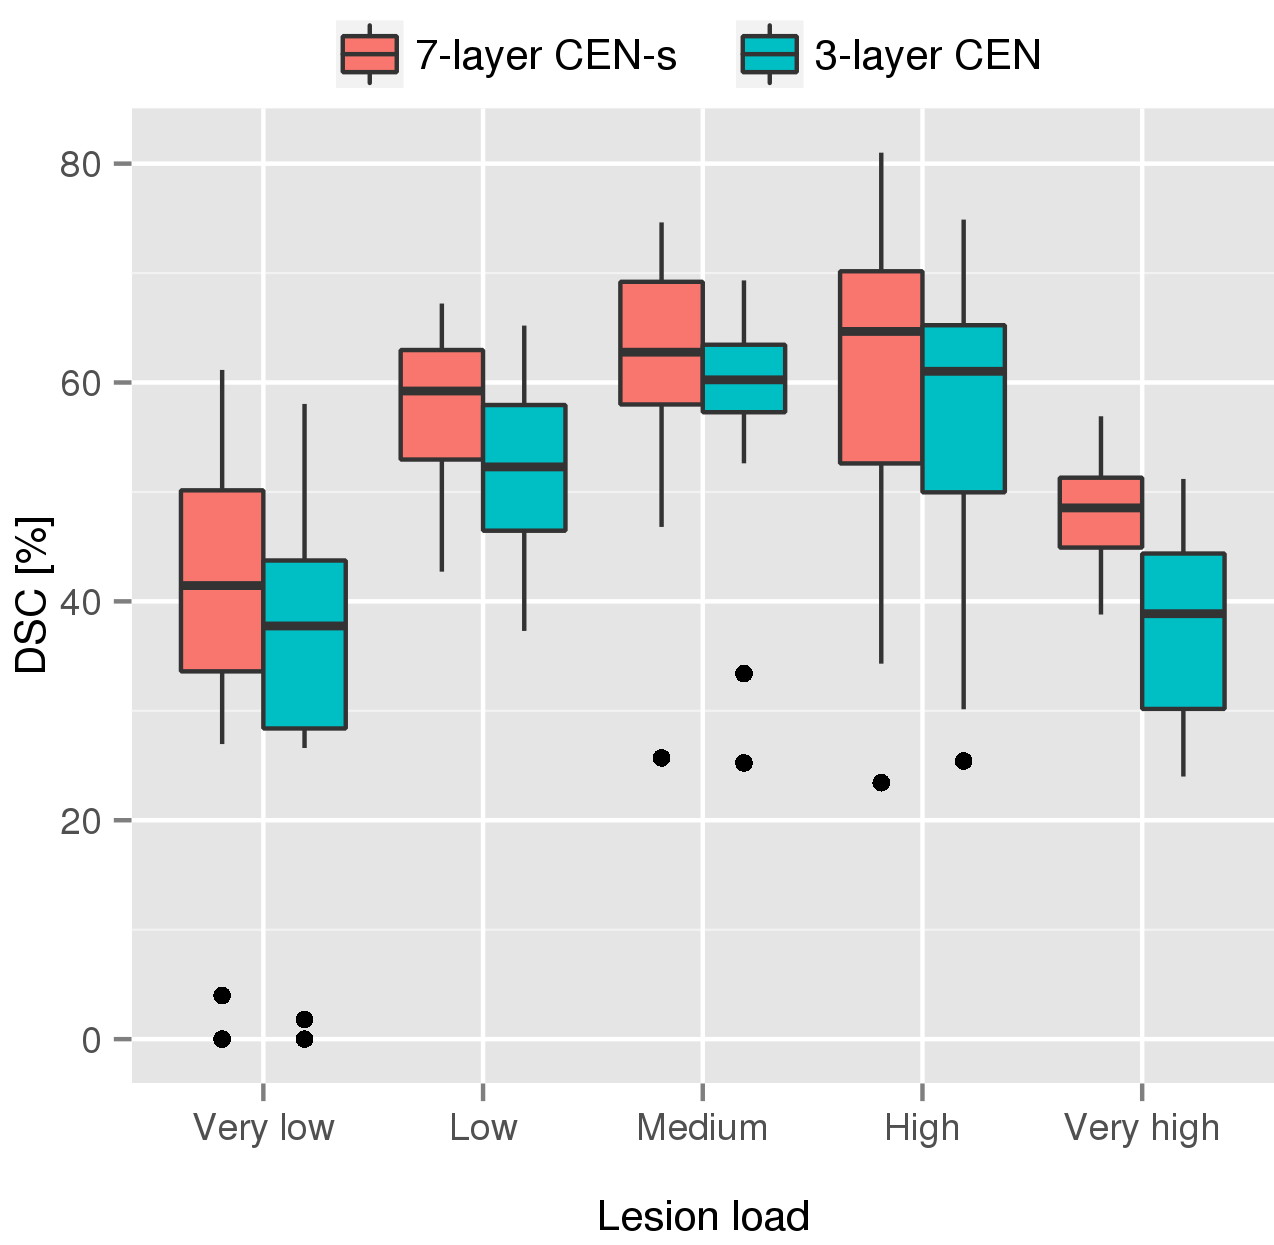
\includegraphics[width=\columnwidth]{figures/boxplot_L1vsL2}

\caption{Comparison of the segmentation accuracy measured by the DSC of a
3-layer CEN and a 7-layer CEN for different lesion load groups. Adding four layers and
shortcut connections improves the performance across all lesion loads, where the
improvements are especially large for scan with large lesion loads, which are
also correlated with an increase in lesion size.}

\label{fig:l1vl2}
\end{figure}

Fig.~\ref{fig:l2vlt} shows a comparison of the 7-layer CEN with shortcut
connections and Lesion-TOADS. The CEN approach performs more consistently
throughout all lesion load groups than Lesion-TOADS, where the improvements are
largest for very low to medium lesion loads. For very high lesion loads,
Lesion-TOADS achieves a higher mean DSC than the CEN approach. However, a
two-sided paired $t$-test yielded that the differences are not statistically
significant ($p\text{-value}=0.2566$). Table~\ref{tab:result2} shows a more
detailed comparison. While the PPV increases consistently with higher lesion
loads for both methods, the TPR is highest for low to medium lesion loads and
decreases again for high to very high lesion loads. This shows the difficulty
for both methods to correctly identify very large lesions that can extend far
into the white matter.

\begin{figure}[tb] \centering
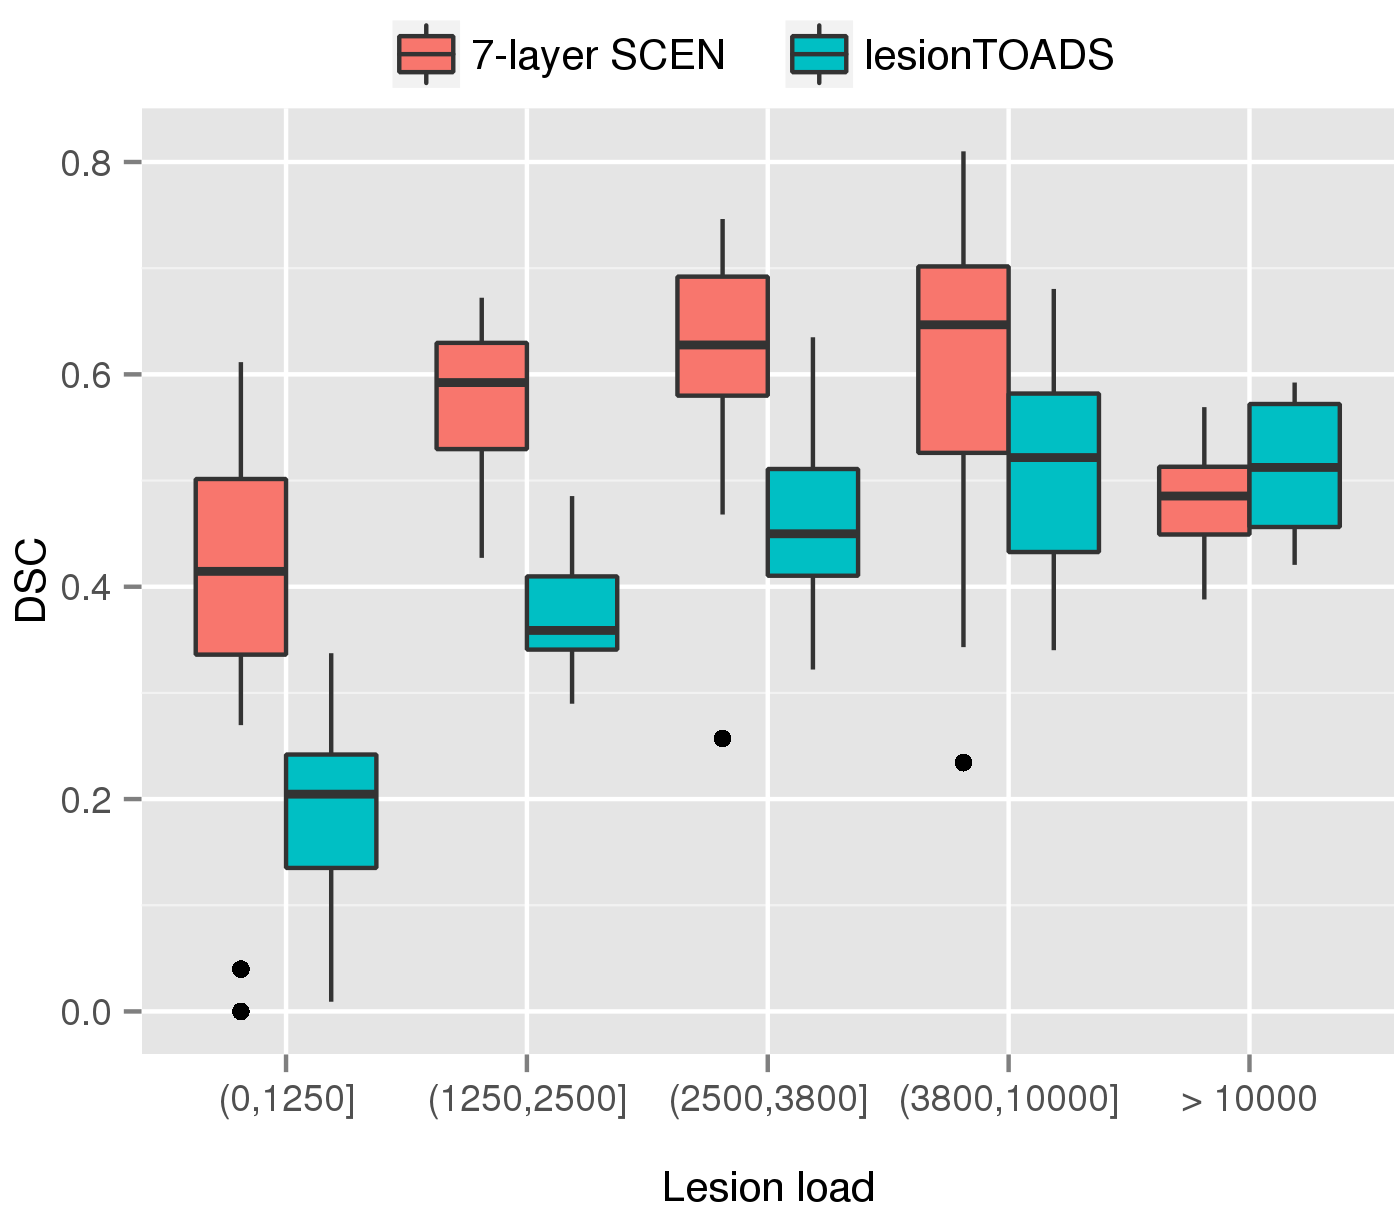
\includegraphics[width=\columnwidth]{figures/boxplot_L2vsLT}
\caption{Comparison of the segmentation accuracy measured by the DSC of
Lesion-TOADS and a 7-layer CEN with shortcut connections for different lesion
loads. The CEN approach is much more sensitive in detecting small lesions, while
still being able to detect large lesions.}
\label{fig:l2vlt}
\end{figure}

\begin{table}
\caption{Comparison of segmentation accuracy for different lesion load
categories.}
\label{tab:result2}
\begin{center}
\begin{tabular}{@{}ccccccc@{}}
\toprule
\multicolumn{1}{@{}l}{Lesion load} & \multicolumn{3}{c}{7-layer SCEN} &
\multicolumn{3}{c@{}}{Lesion-TOADS}
\\
& TPR & PPV & DSC & TPR & PPV & DSC \\
\midrule
\phantom{000}$(0,1250]$\phantom{0} & \num{50.00} & \num{41.15} & \num{39.34} &
\num{49.96} & \num{13.09} & \num{18.86}\\
$(1250,2500]$\phantom{0} & \num{61.92} & \num{59.01} & \num{57.45} & \num{52.39}
& \num{29.95} & \num{37.74}\\
$(2500,3800]$\phantom{0} & \num{57.64} & \num{71.54} & \num{61.31} & \num{54.17}
& \num{41.83} & \num{46.53}\\
$(3800,10000]$ & \num{51.14} & \num{81.11} & \num{60.13} & \num{47.97} &
\num{56.56} & \num{50.76}\\
$> 10000$ & \num{32.82} & \num{91.95} & \num{48.19} & \num{38.88} & \num{74.6} &
\num{50.93}\\
\bottomrule
\end{tabular}
\end{center}
\end{table}

% \begin{itemize}
% \item Have some sample images and discuss what we can see here.
% \end{itemize}

\subsection{Qualitative Results}

A qualitative comparison of segmentation performance for four characteristic
cases is shown in Fig.~\ref{fig:images}. Our method produces segmentations that
are spatially consistent (see Fig.~\ref{fig:images}a), while still being able to
detect small isolated lesions (green circle). Furthermore, our method is able to
learn a wide spectrum of lesion shapes and appearances from training data. This
allows our method to correctly identify multiple different types of MS lesions
(e.g., T1 black holes), which can be challenging to detect for Lesion-TOADS (see
Fig.~\ref{fig:images}b).
Our method uses a combination of automatically learned intensity and appearance
features, which makes it inherently robust to noise as shown in
Fig.~\ref{fig:images}c. Figure~\ref{fig:images}d shows one of the most
challenging cases for our method. Very large lesions might extend beyond the
size of the receptive field of the CEN, which reduces its ability to extract
characteristic lesion features. Consequently, our method might underestimate
the size of very large lesions for some cases.

\begin{figure*}
%\centering
\hspace*{-5pt}
\subfloat[Spatially consistent segmentation] {
\begin{tikzpicture}[node distance=1.5cm and 0.2\columnwidth,
  font=\footnotesize, on grid]
  
\node[,inner sep=0] (image) {
  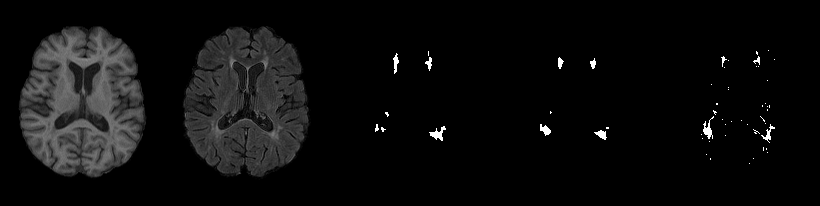
\includegraphics[width=\columnwidth]{figures/p17s29_noisy_lesionTOADS} };
\node[above=of image] (gt) {\phantom{g}Ground truth\phantom{g}};
\node[left=of gt] (flair) {\phantom{g}FLAIR\phantom{g}};
\node[left=of flair] {T1-weighted};
\node[right=of gt,align=center] (cen) {\phantom{g}Our method\phantom{g}};
\node[right=of cen,align=center] {Lesion-\\ TOADS};

\draw[green, thick] (-7pt,-3.5pt) circle (3pt);
\begin{scope}[xshift=0.2\columnwidth]
\draw[green, thick] (-7pt,-3.5pt) circle (3pt);
\end{scope}

\end{tikzpicture}
}
\subfloat[Can handle multiple types of lesions (e.g., T1 black holes)
correctly] {
\begin{tikzpicture}[node distance=1.5cm and 0.2\columnwidth,
  font=\footnotesize, on grid]
  
\node[,inner sep=0] (image) {
  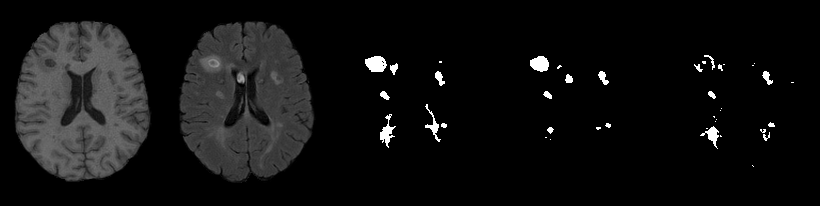
\includegraphics[width=\columnwidth]{figures/p36s30_blackhole}};
\node[above=of image] (gt) {\phantom{g}Ground truth\phantom{g}};
\node[left=of gt] (flair) {\phantom{g}FLAIR\phantom{g}};
\node[left=of flair] {T1-weighted};
\node[right=of gt,align=center] (cen) {\phantom{g}Our method\phantom{g}};
\node[right=of cen,align=center] {Lesion-\\ TOADS};

\draw[red,thick] (-10pt,12pt) circle (7pt);
\begin{scope}[xshift=-0.2\columnwidth]
\draw[red,thick] (-10pt,12pt) circle (7pt);
\end{scope}
\begin{scope}[xshift=-0.4\columnwidth]
\draw[red,thick] (-10pt,12pt) circle (7pt);
\end{scope}
\begin{scope}[xshift=0.2\columnwidth]
\draw[red,thick] (-10pt,12pt) circle (7pt);
\end{scope}
\begin{scope}[xshift=0.4\columnwidth]
\draw[red,thick] (-10pt,12pt) circle (7pt);
\end{scope}

\end{tikzpicture}
}\\
\hspace*{-5pt}
\subfloat[Robust to noise] {
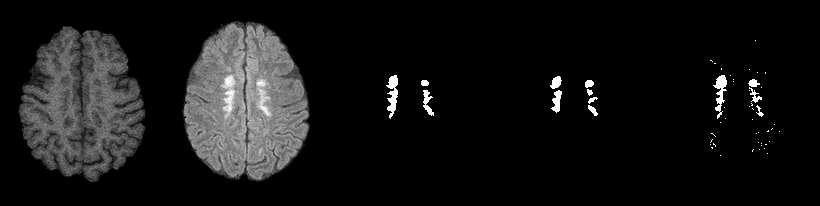
\includegraphics[width=\columnwidth]{figures/p15s34_robust_to_noise3}
}
\subfloat[Underestimates very large lesions] {
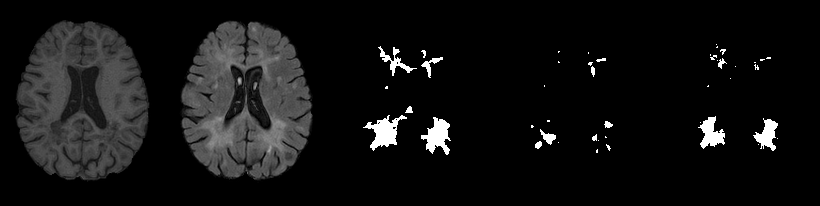
\includegraphics[width=\columnwidth]{figures/p54s32_large_lesions}
}

\caption{Four cases illustrating the strengths and weaknesses of our method
compared to Lesion-TOADS. Our method is able a) to produce spatially consistent
segmentations, b) to handle multiple different types of lesions correctly (e.g.,
T1 black holes), and c) is inherently robust to noise. (d) Our method
might underestimate the size of very large lesions for some cases.}

\label{fig:images}
\end{figure*}

\begin{comment}
\subsection{BioMS Data Set}

\begin{table}
\caption{Training results on the BioMS data set using 150 and 250 images for
training.}
\begin{center}
\begin{tabular}{llcc}
\toprule
Pre-training & Fine-tuning & Training DSC & Test DSC \\
\midrule
With dropout & Hessian-free (150) & 67.1 & 61.7 \\
With dropout & Hessian-free (250) & 68.0 & 62.8 \\
Without dropout & Hessian-free (150) & 66.5 & 61.7 \\
With dropout & AdaDelta (150) & 65.9 & 60.6 \\
Without dropout & AdaDelta (150) & 66.0 & 60.6 \\
\bottomrule
\end{tabular}
\end{center}
Notes: No comparison with
state-of-the-art methods are available here. The effect of dropout in the
pre-training phase on the final result is negligible. Hessian-free is slightly
better than AdaDelta and does not require the tuning of parameters. However,
Hessian-free optimization does not support dropout, which might be important
for regularization when the data set size is small or the number of layers and
filters is high.
\end{table}
\end{comment}

% \subsection{On a small data set}
% 
% Include MICCAI challenge results, because it was a comparison with more methods.

\begin{comment}
\subsection{Evaluation of Training Methods}

We have evaluated the impact of different training and initialization methods on
the performance of the trained network using the example of a 7-layer CEN. The
network architecture is summarized in Table~\ref{tab:arch7}. All methods have
hyperparameters, which can be difficult to choose. To find a good set of
hyperparameters for each algorithm (except for Hessian-free), we first trained
the model for 20 epochs with the hyperparameters shown in
Table~\ref{tab:parameters}. We then used the set of parameters that produced the
lowest error on the training set to further fine-tune the model for 500 epochs.
This tuning procedure favors algorithms that are robust to the choice of the
hyperparameters or can make substantial progress within the first few epochs,
which are both desirable properties of a training method for which
time-consuming parameter tuning using a large number of epochs and
cross-validation is not feasible. As is the case for the training on large data
sets on high-resolution 3D medical images. The hyperparameters of the
Hessian-free optimization are very robust to the choice of input data. We found
that tuning these parameters is not necessary. Another difference of the
Hessian-free optimization compared to the other methods is that HF is able to
make more progress within an epoch, albeit at the cost of more time-consuming
updates. To compensate, we trained HF for only 22 epochs. Parameter estimation
and fine-tuning of the model required 2.9 GB of GPU memory and took
approximately 42 hours on a single NVIDIA GeForce GTX 780 graphics card.
However, once the model has been trained, segmentation of an entire 3D image can
be performed in less than half a seconds.

\begin{table}
\caption{Algorithm parameters}%
\label{tab:parameters}
\begin{center}
\begin{tabular}{@{}lp{0.7\columnwidth}@{}}
\toprule
Algorithm & Parameters \\
\midrule
SGD \cite{LeCun1998} & $\text{learning rate} \in \{\num{e-3}, \num{e-4}, \num{e-5},
\num{e-6}\},\newline \text{momentum} = 0.9$ \\

AdaGrad \cite{duchi2011adaptive} & $\alpha \in \{\num{e-4}, \num{e-5},
\num{e-6}, \num{e-7}\}, \epsilon = \num{e-11}$ \\

Adam \cite{kingma2014adam} & $\alpha \in \{\num{3e-5}, \num{e-5}, \num{e-6},
\num{e-7}\}$, $\beta_1 = 0.1$, \newline $\beta_2 = 0.001$, $\epsilon = \num{e-11}$ \\

AdaDelta \cite{zeiler2012adadelta} & $\epsilon \in \{\num{e-9}, \num{e-10},
\num{e-11}\}, \rho= 0.95$
\\

RMSProp \cite{dauphin2015rmsprop} & $\epsilon \in \{\num{e-4}, \num{e-5},
\num{e-6}, \num{e-7}\}, \alpha = 0.9 $\\

Hessian-free \cite{martens2010deep} & $\lambda_0 = 1, \zeta = 0.9$ \\
\bottomrule
\end{tabular}
\end{center}
Note: Please refer to the respective paper for a detailed description of the
hyperparameters.
\end{table}

Figure~\ref{fig:methods} shows a comparison of Dice similarity coefficients
calculated on the test set after training the 7-layer CEN with different
optimization methods as well as with and without pre-training. The results for
SGD are not included in the figure, because we were not able to find a learning
rate for which SGD can make notable progress.
\begin{itemize}
\item SGD is not included because the training method failed to make notable
progress
\item A possible explanation is that the parameters of different layers vary
greatly in magnitude and therefore require different learning rates
\item However, SGD used the same learning rate for all layers and the tuning
phase was not able to find a learning rate that works for all layers
\item In addition, none of the first-order methods were able to train the
CEN without pre-training, which further highlights the difficulty of training deep
CNNs on sparse segmentations.
\item We found that pre-training is crucial to alleviate the difficulty of
training deep CNNs with very unbalanced classes.
\item The training algorithms AdaDelta, Adam, Hessian-free and RMSProp perform
roughly the same with only AdaGrad notably worse than the other methods.
\item Hessian-free optimization was the only method that did not require
pre-training, where the results with pre-training are still slightly better than
without pre-training
\end{itemize}  

\begin{figure}[tb]
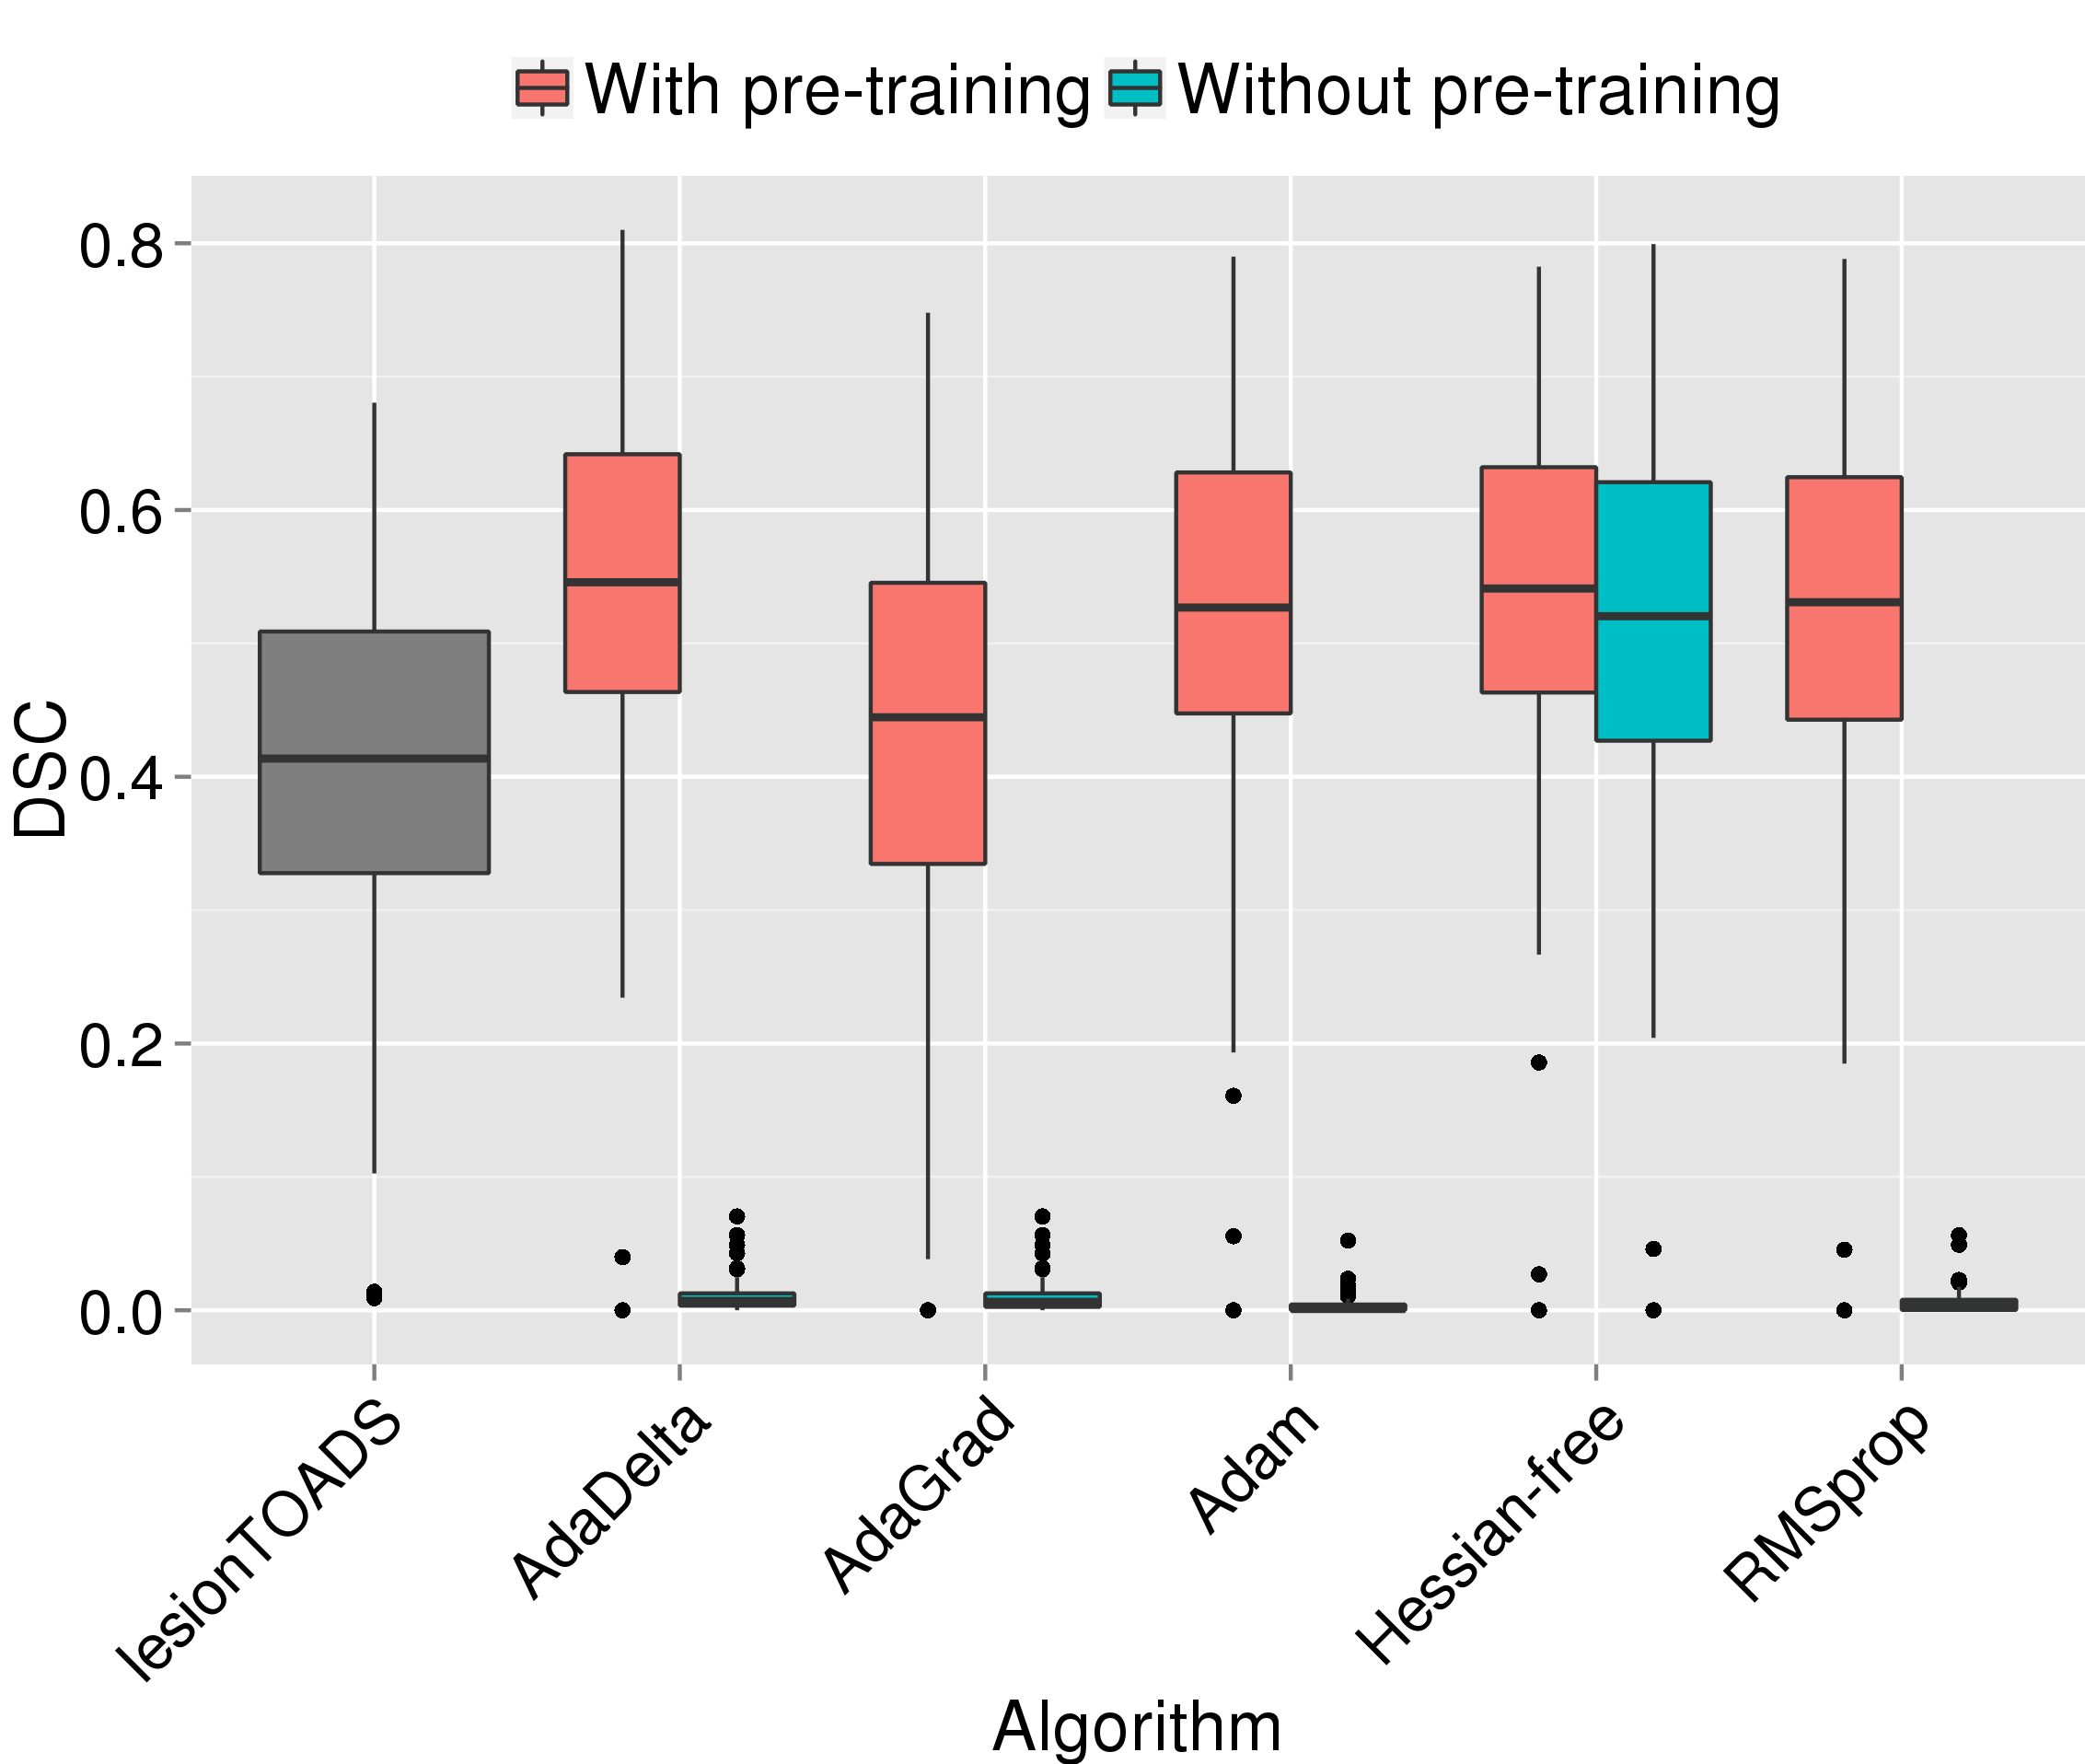
\includegraphics[width=\columnwidth]{figures/methods2}
\caption{Comparison of different training methods with pre-training (left) and
without pre-training (right). Hessian-free is the only method that does not
require pre-training to train the model. With pre-training, AdaDelta, Adam,
Hessian-free, and RMSprop consistently learn models that perform significantly
better than lesionTOADS.}
\label{fig:methods}
\end{figure}

A more detailed comparison of the 7-layer CEN trained with different
optimization algorithms and lesionTOADS is summarized in Table~\ref{tab:results1}.
\begin{itemize}
\item TPR is comparable to lesionTOADS, whereby only the CEN trained with
AdaDelta is able to achieve a higher TPR than lesionTOADS
\item Advantage of CEN model is the much reduces number of false positives,
which results in a significantly higher PPV.
\item All methods, except for AdaGrad, outperform lesionTOADS in terms of the
DCS by more than \SI{10}{\percent}. The best performing method achieves a DSC of
\num{54.02} compared to a DSC of \num{40.04} achieved by lesionTOADS on this
challenging data set.
\end{itemize}

\begin{table}
\sisetup{separate-uncertainty=true,detect-weight=true,detect-inline-weight=math}
\begin{center}
\caption{Comparison of the segmentation accuracy of a 7-layer CEN trained with
different algorithms and lesionTOADS}
\label{tab:results1}
\begin{tabular}{@{}lccc@{}}
\toprule
Algorithm & TPR [\%] & PPV [\%] & DSC [\%] \\
\midrule
AdaDelta & \textbf{\num{52.75+-20.31}} & \num{66.58+-20.71} &
\textbf{\num{54.02+-15.24}} \\
AdaGrad & \num{42.14+-18.88} & \num{54.65+-20.24} & \num{43.21+-15.05} \\
Adam & \num{47.41+-18.96} & \textbf{\num{70.33+-20.98}} & \num{51.93+-15.08} \\
Hessian-free & \num{49.21+-18.76} & \num{68.33+-21.12} & \num{52.65+-15.09} \\
RMSprop & \num{47.9+-20.53} & \num{69.12+-20.78} & \num{51.46+-15.77} \\[0.4em]
lesionTOADS & \num{49.83+-14.79} & \num{39.86+-20.95} & \num{40.04+-14.86} \\
\bottomrule
\end{tabular}
\end{center}
Note: The table shows the mean and standard deviation of the true positive rate
(TPR), positive predictive value (PPV), and Dice similarity coefficient (DSC).
All experiments were performed with pre-training and evaluated on the test set.
\end{table}

\subsection{Evaluation of Network Architectures}

In a second experiment, we evaluated the impact of the network architecture on
the segmentation performance. Therefore, we have trained different networks with
varying number of layers and with and without shortcut connections between the
convolutional and deconvolutional pathway. Table~\ref{tab:arch15} shows the
parameters of a 15-layer CEN. We have used the same parameters for the 11-layer,
7-layer, and 3-layer CENs with the respective layers removed.
\begin{itemize}
\item Shortcut connections are increasingly more important with increasing
depth of the network
\item The DSC decreases with depth without shortcut while it increases with
shortcuts
\item After 11 layers, the network performance does not increase on the test set
as the network starts to overfit more
\item Either more training data or better regularization methods are needed to
train very deep models
\end{itemize}

\begin{table}[tb]
\caption{Parameters of the 15 layers of the CENs used to evaluate different
network architectures.}
\label{tab:arch15}
\begin{center}
\begin{tabular}{@{}lccr@{}}
\toprule
Layer type & Kernel size & Filters & \multicolumn{1}{c}{Image size} \\
\midrule
Input & --- & --- & \num{164x206x52x2}\phantom{0} \\
Convolutional & \num{9x9x5x2} & 32 & \num{156x198x48x32} \\
Average Pooling & \num{2x2x2} & --- & \num{78x99x24x32} \\
Convolutional & \num{9x10x5x32} & 32 & \num{70x90x20x32} \\
Average Pooling & \num{2x2x1} & --- & \num{35x45x20x32} \\
Convolutional & \num{8x10x5x32}  & 32 & \num{28x36x16x32} \\
Average Pooling & \num{2x2x1} & --- & \num{14x18x16x32} \\
Convolutional & \num{7x11x9x32}  & 32 & \num{8x8x8x32} \\
Deconvolutional & \num{7x11x9x32}  & 32 & \num{14x18x16x32} \\
Unpooling & \num{2x2x1}       & --- & \num{28x36x16x32} \\
Deconvolutional & \num{8x10x5x32} & 32 & \num{35x45x20x32} \\
Unpooling & \num{2x2x1}       & --- & \num{70x90x20x32} \\  
Deconvolutional & \num{9x10x5x32} & 32 & \num{78x99x24x32} \\
Unpooling & \num{2x2x2} & --- & \num{156x198x48x32} \\
Deconvolutional & \num{9x9x5x32} & 1 & \num{164x206x52x1}\phantom{0} \\
\bottomrule
\end{tabular}
\end{center}
Note: Networks with fewer layer use the same parameters as the 15-layer
CEN, where the missing layers are simply removed.
\end{table}

Analysis of different training set sizes
\begin{itemize}
\item Varying number of training samples
\item With dropout and without (regularization)
\item Performed on most promising architecture
\item Possible outcome: to harsh regularization decreases performance when
enough training data is available but improves performance for small data sets
due to the reduction of overfitting
\end{itemize}
\end{comment}

% \begin{table}
% \caption{Preliminary segmentation results on the Bravo data set.}
% \begin{center}
% \begin{tabular}{lc}
% \toprule
% Method & Training and test DSCs \\
% \midrule
% Input pre-training, 1-layer CNN &  41.63 / 42.76 \\[0.25em]
% No pre-training, 2-layer CNN & 51.88 / 46.93 \\
% Joint pre-training, 2-layer CNN & 44.52 / 43.82 \\
% Input pre-training, 2-layer CNN & 51.02 / 46.58 \\[0.25em]
% Input pre-training, 4-layer CNN & 59.60 / 46.14 \\[0.25em]
% Lesion-TOADS & \phantom{00.}--- / 34.87 \\
% \bottomrule
% \end{tabular}
% \end{center}
% Note: All tests were performed with Hessian-free optimization. Pre-training was
% always performed with dropout.
% \end{table}

\begin{comment}


To allow for a direct comparison with state-of-the-art lesion segmentation
methods, we evaluated our method on the FLAIR, T1-, and T2-weighted MRIs of the
20 publicly available labeled cases from the MS lesion segmentation challenge
2008 \cite{styner20083d}, which we downsampled from the original isotropic voxel
size of \SI{0.5}{\cubic\milli\metre} to an isotropic voxel size of
\SI{1.0}{\cubic\milli\metre}. In addition, we evaluated our method on an
in-house data set from an MS clinical trial of 500 subjects split equally into
training and test sets. The images were acquired from 45 different scanning
sites. For each subject, the data set contains T2- and PD-weighted MRIs with a
voxel size of \SI{0.937x0.937x3.000}{\milli\metre}. The main preprocessing steps
included rigid intra-subject registration, brain extraction, intensity
normalization, and background cropping.

We used a CEN with 32 filters and filter sizes of \num{9x9x9} and \num{9x9x5}
voxels for the challenge and in-house data sets, respectively. Training on a
single GeForce GTX 780 graphics card took between 6 and 32 hours per model
depending on the training set size. However, once the network is trained,
segmentation of trimodal 3D volumes with a resolution of, e.g.,
\num{159x201x155} voxels can be performed in less than one second. As a
rough\footnote{Ciresan et al. used a more complex network that is composed of 11
layers. However, their network was trained on much smaller images, which roughly
compensates for the increased complexity.} comparison, Ciresan et al.
\cite{Ciresan2012} reported that their patch-based method required 10 to 30
minutes to segment a single 2D image with a resolution of \num{512x512} voxels
using four graphics cards, which demonstrates the large speed-ups gained by
processing entire volumes.

% \begin{figure}[tb]
% \centering
% \small
% \def\MRIwidth{0.15\textwidth}
% 
% \begin{tikzpicture} 
% \tikzstyle{leftlabel}=[rotate=90, align=center,overlay,above]
% 
% \matrix [matrix of nodes, nodes={anchor=center, inner sep=1pt}] {
%         &[4pt] FLAIR & T1w & T2w & Ground truth & Our method \\[4pt]
% \node[leftlabel] {CHB\,07\\(DSC\,=\,\SI{60.58}{\percent})}; &
% 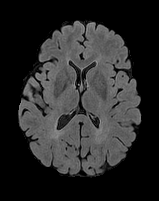
\includegraphics[width=\MRIwidth]{figures/CHB07-FLAIR-s88} &
% 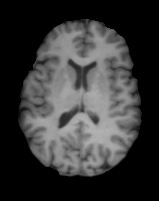
\includegraphics[width=\MRIwidth]{figures/CHB07-T1w-s88} &
% 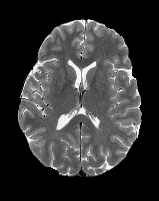
\includegraphics[width=\MRIwidth]{figures/CHB07-T2w-s88} &
% 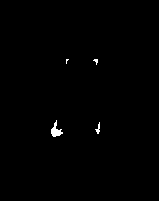
\includegraphics[width=\MRIwidth]{figures/CHB07-gold-s88} &
% 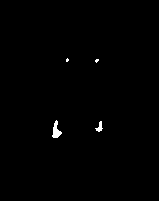
\includegraphics[width=\MRIwidth]{figures/CHB07-pred-s88} \\
% \node[leftlabel] {CHB\,04\\(DSC\,=\,\SI{61.37}{\percent})}; &
% 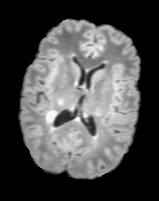
\includegraphics[width=\MRIwidth]{figures/CHB04-FLAIR-s85} &
% 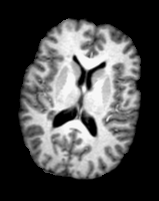
\includegraphics[width=\MRIwidth]{figures/CHB04-T1w-s85} &
% 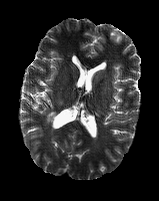
\includegraphics[width=\MRIwidth]{figures/CHB04-T2w-s85} &
% 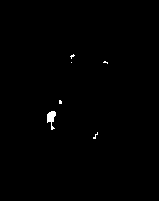
\includegraphics[width=\MRIwidth]{figures/CHB04-gold-s85} &
% 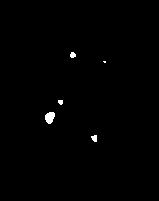
\includegraphics[width=\MRIwidth]{figures/CHB04-pred-s85} \\
% \node[leftlabel] {UNC\,09\\(DSC\,=\,\SI{9.01}{\percent})}; &
% 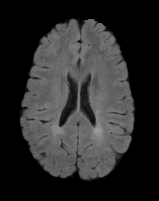
\includegraphics[width=\MRIwidth]{figures/UNC09-FLAIR-s89} &
% 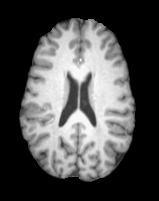
\includegraphics[width=\MRIwidth]{figures/UNC09-T1w-s89} &
% 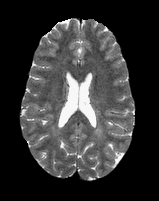
\includegraphics[width=\MRIwidth]{figures/UNC09-T2w-s89} &
% 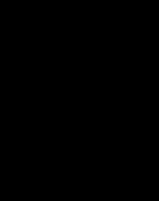
\includegraphics[width=\MRIwidth]{figures/UNC09-gold-s89} &
% 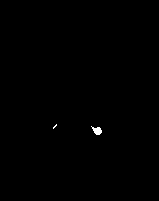
\includegraphics[width=\MRIwidth]{figures/UNC09-pred-s89} \\
% };
% \end{tikzpicture}
% 
% \caption{Example segmentations of our method for three different subjects from
% the challenge data set. Our method performed well and consistently despite the
% large contrast differences seen between the first two rows. In the third row,
% our method also segmented lesions that have similar contrast, but these regions
% had not been identified as lesions by the manual rater, which highlights the
% difficulty in distinguishing focal lesions from diffuse damage, even for
% experts.}
% 
% \label{fig:segmentation}
% \end{figure}

We evaluated our method on the challenge data set using 5-fold
cross-valida\-tion and calculated the true positive rate (TPR), positive
predictive value (PPV), and Dice similarity coefficient (DSC) between the
predicted segmentations and the resampled ground truth.
Figure~\ref{fig:segmentation} shows a comparison of three subjects from the
challenge data set. The first two rows show the FLAIR, T1w, T2w, ground truth
segmentations, and predicted segmentations of two subjects with a DSC of
\SI{60.58}{\percent} and \SI{61.37}{\percent}. Despite the large contrast
differences between the two subjects, our method performed well and
consistently, which indicates that our model was able to learn features that are
robust to a large range of intensity variations. The last row shows a subject
with a DSC of \SI{9.01}{\percent}, one of the lowest DSC scores from the data
set. Our method segmented lesions that have similar contrast to the other two
subjects, but these regions were not classified as lesions by the manual rater.
This highlights the difficulty of manual lesion segmentation, as the difference
between diffuse white matter pathology and focal lesions is often indistinct. A
quantitative comparison of our method with other state-of-the-art methods is
summarized in Table~\ref{tab:state}. Our method outperforms the winning method
(Souplet et al. \cite{souplet2008}) of the MS lesion segmentation challenge 2008
and the currently best unsupervised method reported on that data set (Weiss et
al. \cite{weiss2013}) in terms of mean TPR and PPV. Our method performs
comparably to a current method (Geremia et al. \cite{geremia2010}) that uses a
carefully designed set of features specifically designed for lesion
segmentation, despite our method having learned its features solely from a
relatively small training set.

\begin{table}[tb]
\def\tabspace{12pt}

\caption{Comparison of our method with state-of-the-art lesion segmentation
methods in terms of mean TPR, PPV, and DSC. Our method performs comparably to
the best methods reported on the MS lesion segmentation challenge data set.}

\label{tab:state}
\centering
\begin{tabular}{l%
@{\hspace{\tabspace}}S[table-format=2.2]
@{\hspace{\tabspace}}S[table-format=2.2]
@{\hspace{\tabspace}}S[table-format=2.2]
}
\toprule
Method & {TPR} & {PPV} & {DSC} \\ 
\midrule
Souplet et al. \cite{souplet2008} & 20.65 & 30.00 & {---} \\ 
Weiss et al. \cite{weiss2013} & 33.00 & 36.85 & 29.05 \\ 
Geremia et al. \cite{geremia2010} & 39.85 & 40.35 & {---}  \\
Our method & 39.71 & 41.38 & 35.52 \\
\bottomrule
\end{tabular}
\end{table}

To evaluate the impact of the training set size on the segmentation performance,
we trained our model on our in-house data set with a varying number of training
samples and calculated the mean DSC on the training and test sets as illustrated
in Fig.~\ref{fig:bioms}. For small training sets, there is a large difference
between the DSCs on the training and test sets, which indicates that the
training set is too small to learn a representative set of features. At around
100 samples, the model becomes stable in terms of test performance and the small
difference between training and test DSCs, indicating that overfitting of the
training data is no longer occurring. With 100 training subjects, our method
achieves a mean DSC on the test set of \SI{57.38}{\percent}, which shows that
the segmentation accuracy can be greatly improved compared to the results on the
challenge data set, when a representative training set is available.

\begin{figure}[tb]
\centering
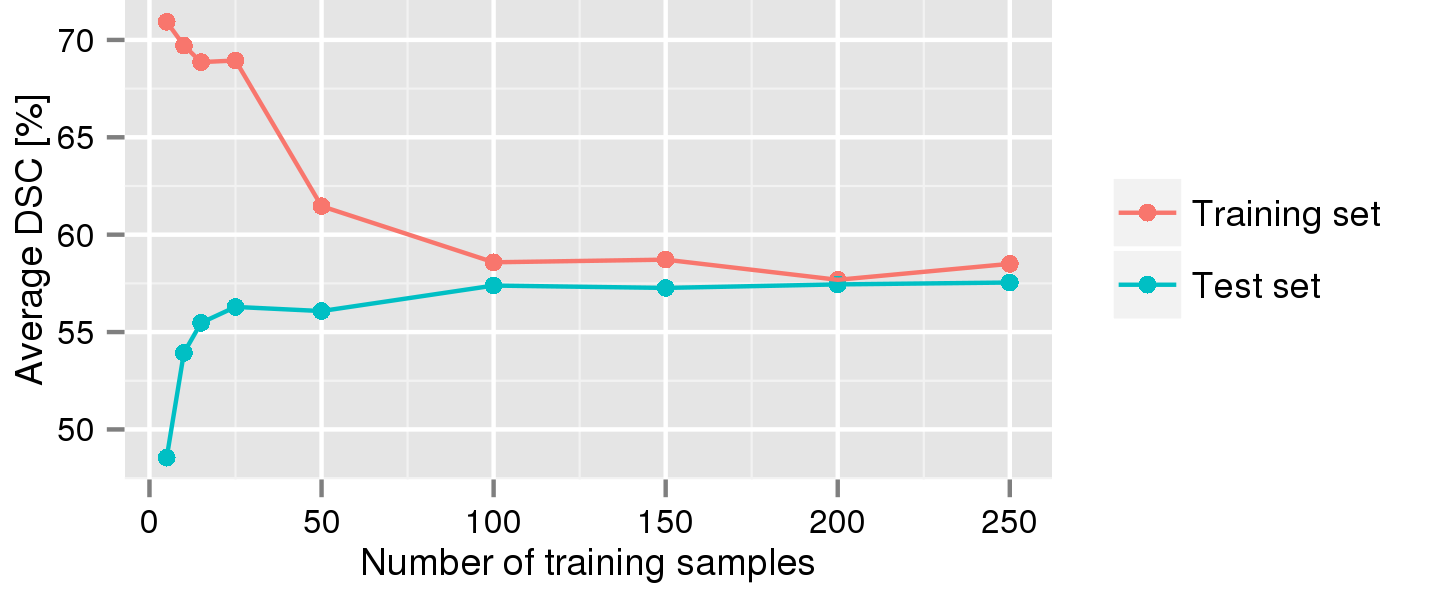
\includegraphics[width=0.78\textwidth]{figures/train_count}

\caption{Comparison of DSC scores calculated on the training and test sets for
varying numbers of training samples. At around 100 samples, the model becomes
stable in terms of test performance and the small difference between training
and test DSCs, indicating that overfitting of the training data no longer
occurs.}
\label{fig:bioms}
\end{figure}

\end{comment}

\section{Conclusions}

We have introduced a new method for the automatic segmentation of MS lesions
based on convolutional encoder networks. The joint training of the feature
extraction and prediction layers with a novel objective function allows for the
automatic learning of features that are tuned for a given combination of image
types and a segmentation task with very unbalanced classes.
We have evaluated our method on two data sets showing that approximately 100
images are required to train the model without overfitting but even when only a
relatively small training set is available, the method still performs comparably
to the state-of-the-art algorithms. For future work, we plan to increase the
depth of the network, which would allow the learning of a set of hierarchical
features. This could further improve segmentation accuracy, but may require
larger training sets. We would also like to investigate the use of different
objective functions for training based on other measures of segmentation
performance.

\section*{Acknowledgements}
\label{sec:achnowledge}
This work was supported by Natural Sciences and Engineering Research Council of
Canada and the Milan and Maureen Ilich Foundation.


\bibliographystyle{splncs}
\bibliography{bib}

\end{document}
